\subsection{Cơ chế chính của trò chơi}
\subsubsection{Cơ chế chọn thẻ bài}
Khi đến lượt của người chơi, người chơi có thể di chuột vào thẻ bài để có thể chọn thẻ bài mình muốn sử dụng, nếu thẻ đó có thể sử dụng được thì sẽ có viền màu vàng và di chuyển lên trên, còn nếu không sử dụng được thì sẽ có viền màu đỏ và đứng im không di chuyển.
\begin{figure} [H]
    \centering
    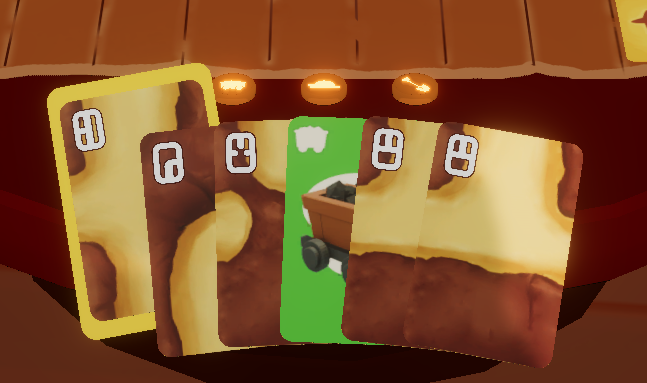
\includegraphics[width=0.5\linewidth]{10.Kết quả//images/SelectCard.png}
    \caption{Screenshot chọn thẻ bài dùng được}
    \label{fig:placeholder}
\end{figure}
\begin{figure}[H]
    \centering
    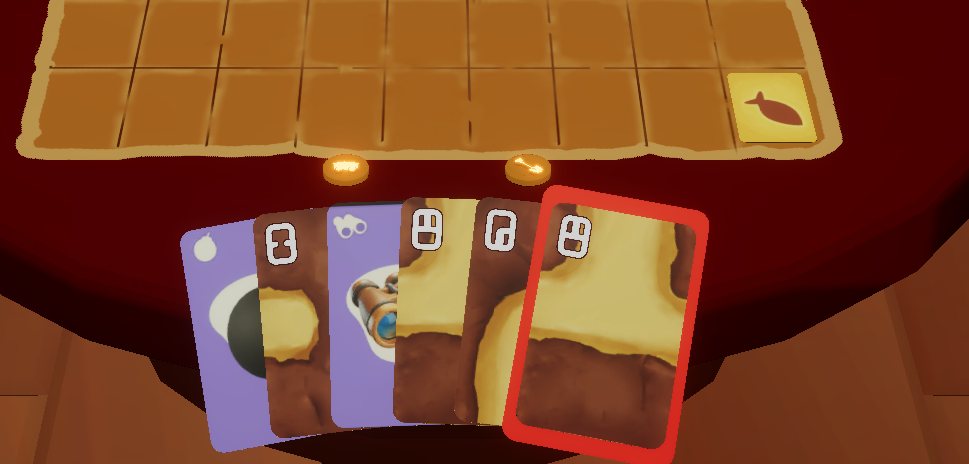
\includegraphics[width=0.5\linewidth]{10.Kết quả//images/CannotHoverCard.png}
    \caption{Screenshot chọn thẻ bài không dùng được}
    \label{fig:placeholder}
\end{figure}
Khi nhấn vào sử dụng thẻ bài nào thì thẻ bài đó sẽ di chuyển xuống dưới bàn và hiển thị những vị trí có thể đặt được, người chơi chỉ cần di chuyển chuột đến vị trí đó rồi nhấn chuột trái là có thể sử dụng. Ở đây chia ra làm 4 loại thẻ bài:
\begin{itemize}
    \item \textbf{Thẻ đường} sẽ đặt lên những vị trí có thể đặt dựa trên trạng thái board hiện tại và đường đi của thẻ.
    \item \textbf{Thẻ hành động} như phá, hồi phục công cụ, dùng khiên thì sẽ cần phải di chuột vào người chơi.
    \item \textbf{Thẻ liên quan đến kho báu} như xem thẻ kho báu, đổi vị trí kho báu thì cần di chuột vào 1 trong 3 thẻ kho báu ở trên bàn.
    \item Riêng \textbf{Thẻ hành động đặt bom} thì cần phải di chuột vào những thẻ đường đã được đặt xuống trừ thẻ bắt đầu và thẻ kho báu.
\end{itemize}    
\begin{figure} [H]
    \centering
    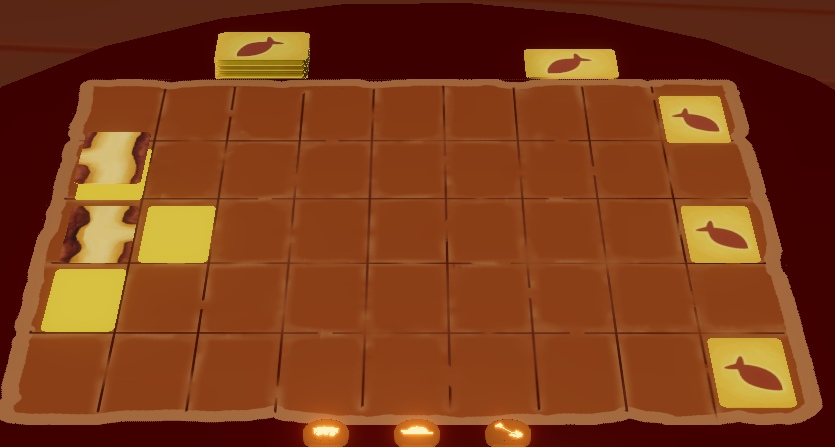
\includegraphics[width=0.5\linewidth]{10.Kết quả//images/PlaceCard.png}
    \caption{Screenshot đặt card xuống}
\end{figure}
\begin{figure}[H]
    \centering
    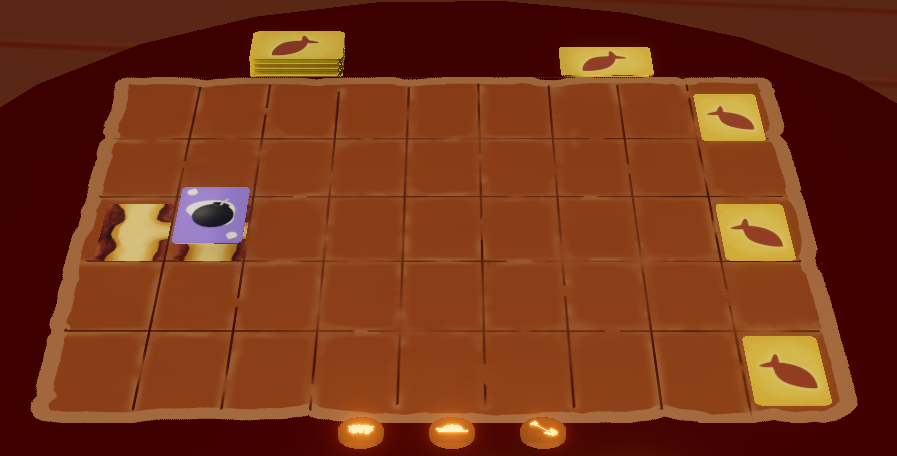
\includegraphics[width=0.5\linewidth]{10.Kết quả//images/HoverBomb.png}
    \caption{Screenshot chọn vị trí đặt bom}
    \label{fig:placeholder}
\end{figure}
\begin{figure}[H]
    \centering
    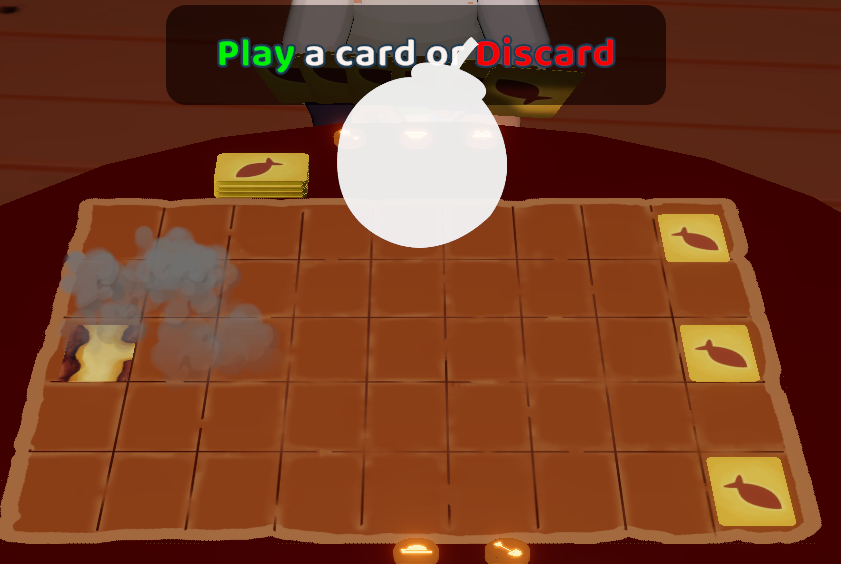
\includegraphics[width=0.5\linewidth]{10.Kết quả//images/BombUsed.png}
    \caption{Screenshot sử dụng bom}
    \label{fig:placeholder}
\end{figure}
\begin{figure}[H]
    \centering
    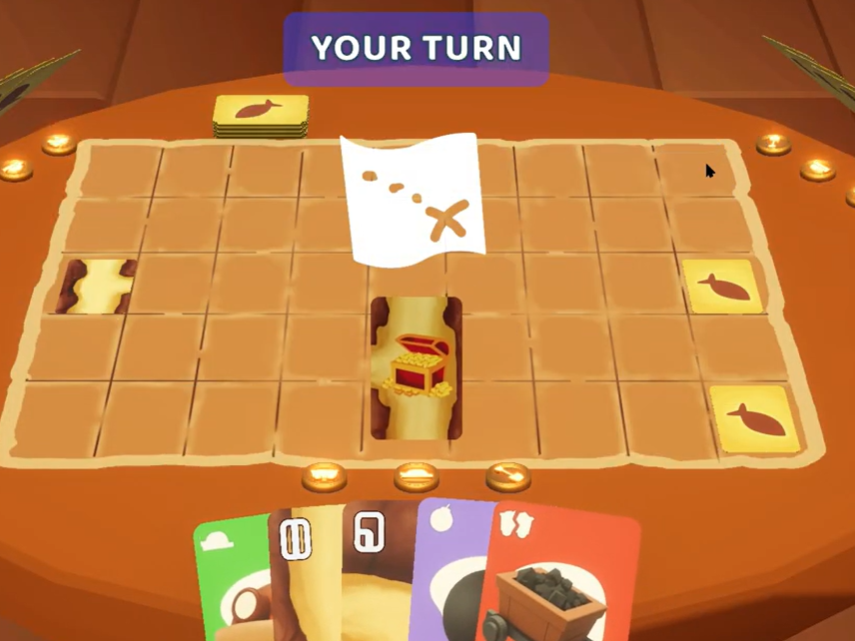
\includegraphics[width=0.5\linewidth]{10.Kết quả//images/MapUsed.png}
    \caption{Screenshot sử dụng thẻ xem kho báu}
    \label{fig:placeholder}
\end{figure}
\begin{figure}[H]
    \centering
    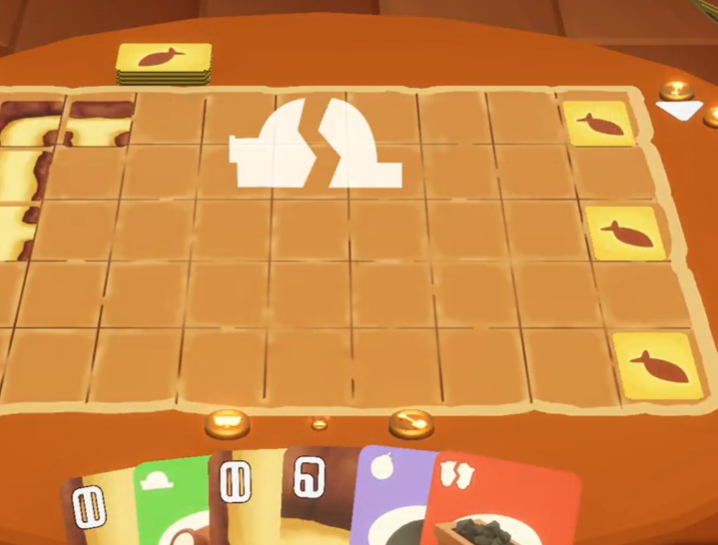
\includegraphics[width=0.5\linewidth]{10.Kết quả//images/BreakTool.png}
    \caption{Screenshot sử dụng thẻ phá công cụ}
    \label{fig:placeholder}
\end{figure}
\begin{figure}[H]
    \centering
    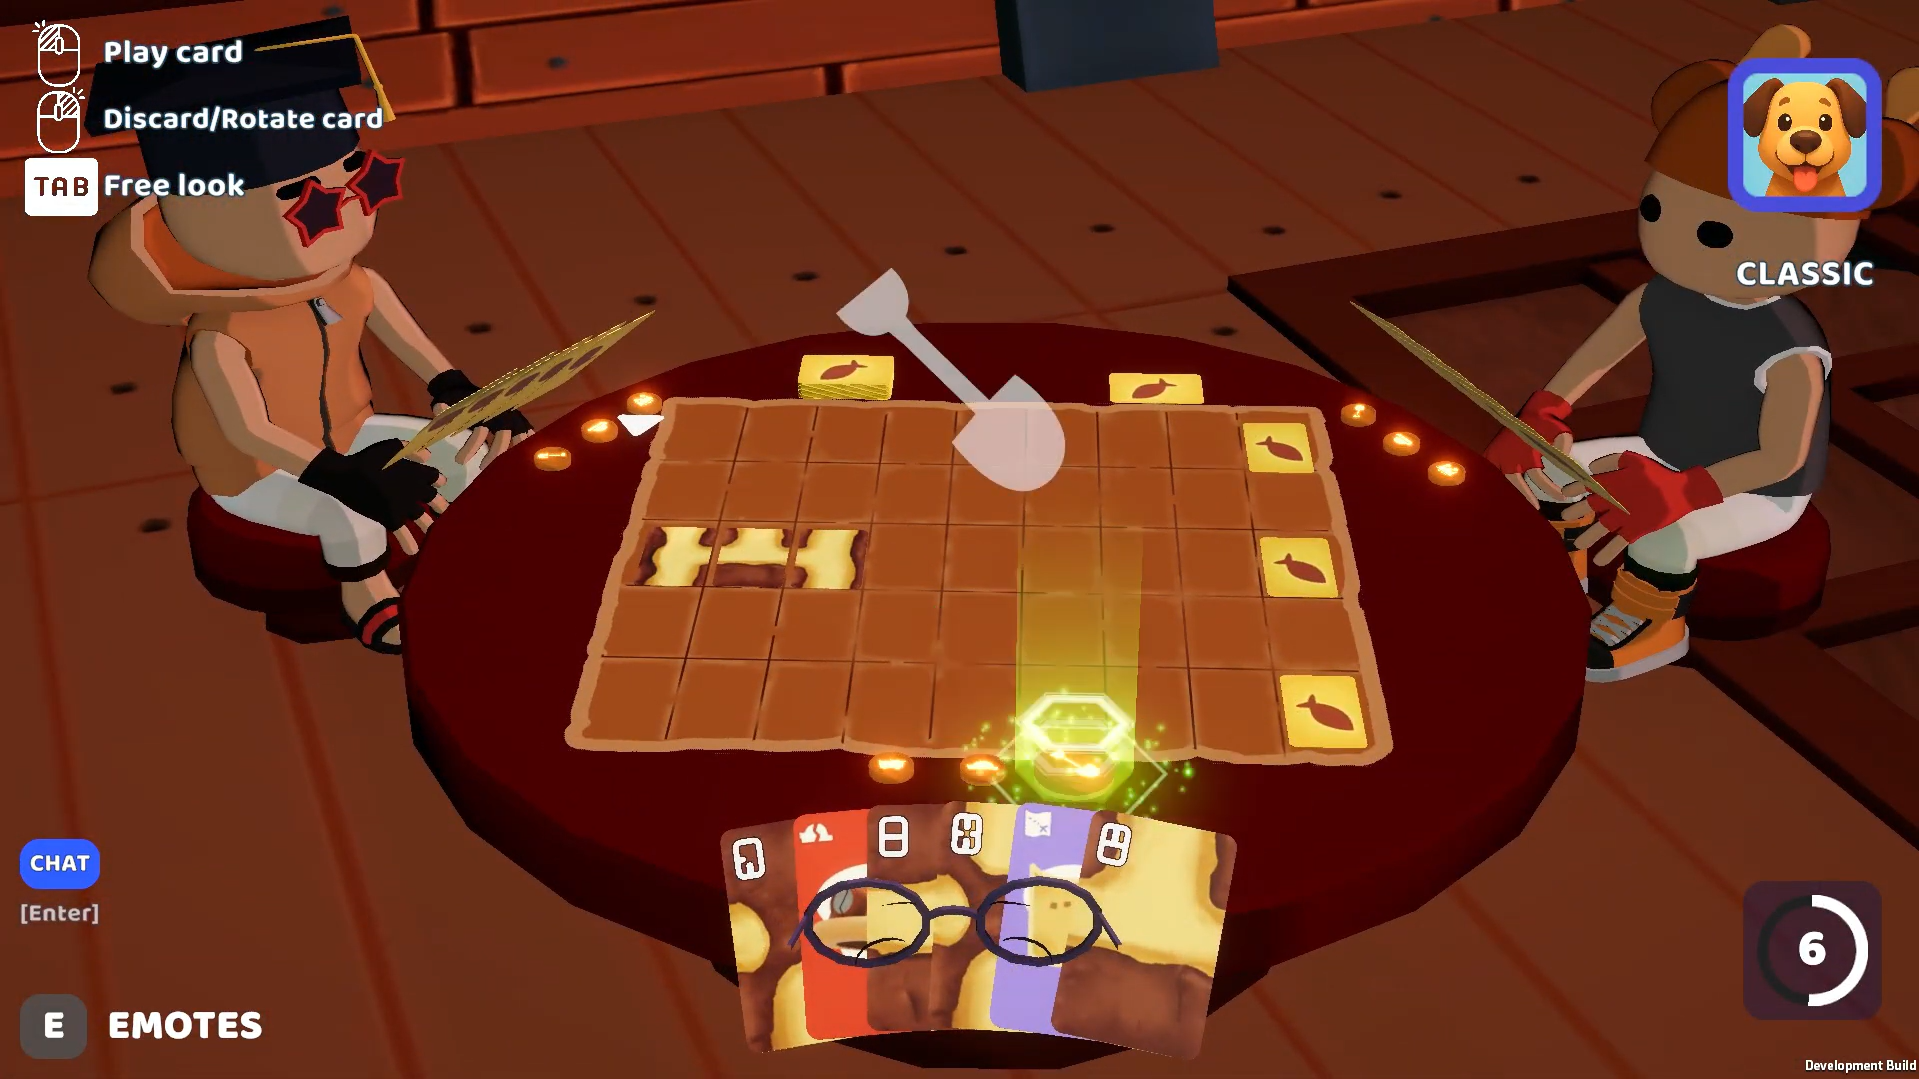
\includegraphics[width=0.5\linewidth]{10.Kết quả//images/ReviveTool.png}
    \caption{Screenshot sử dụng thẻ chức năng hồi phục công cụ}
    \label{fig:placeholder}
\end{figure}

\begin{figure}[H]
    \centering
    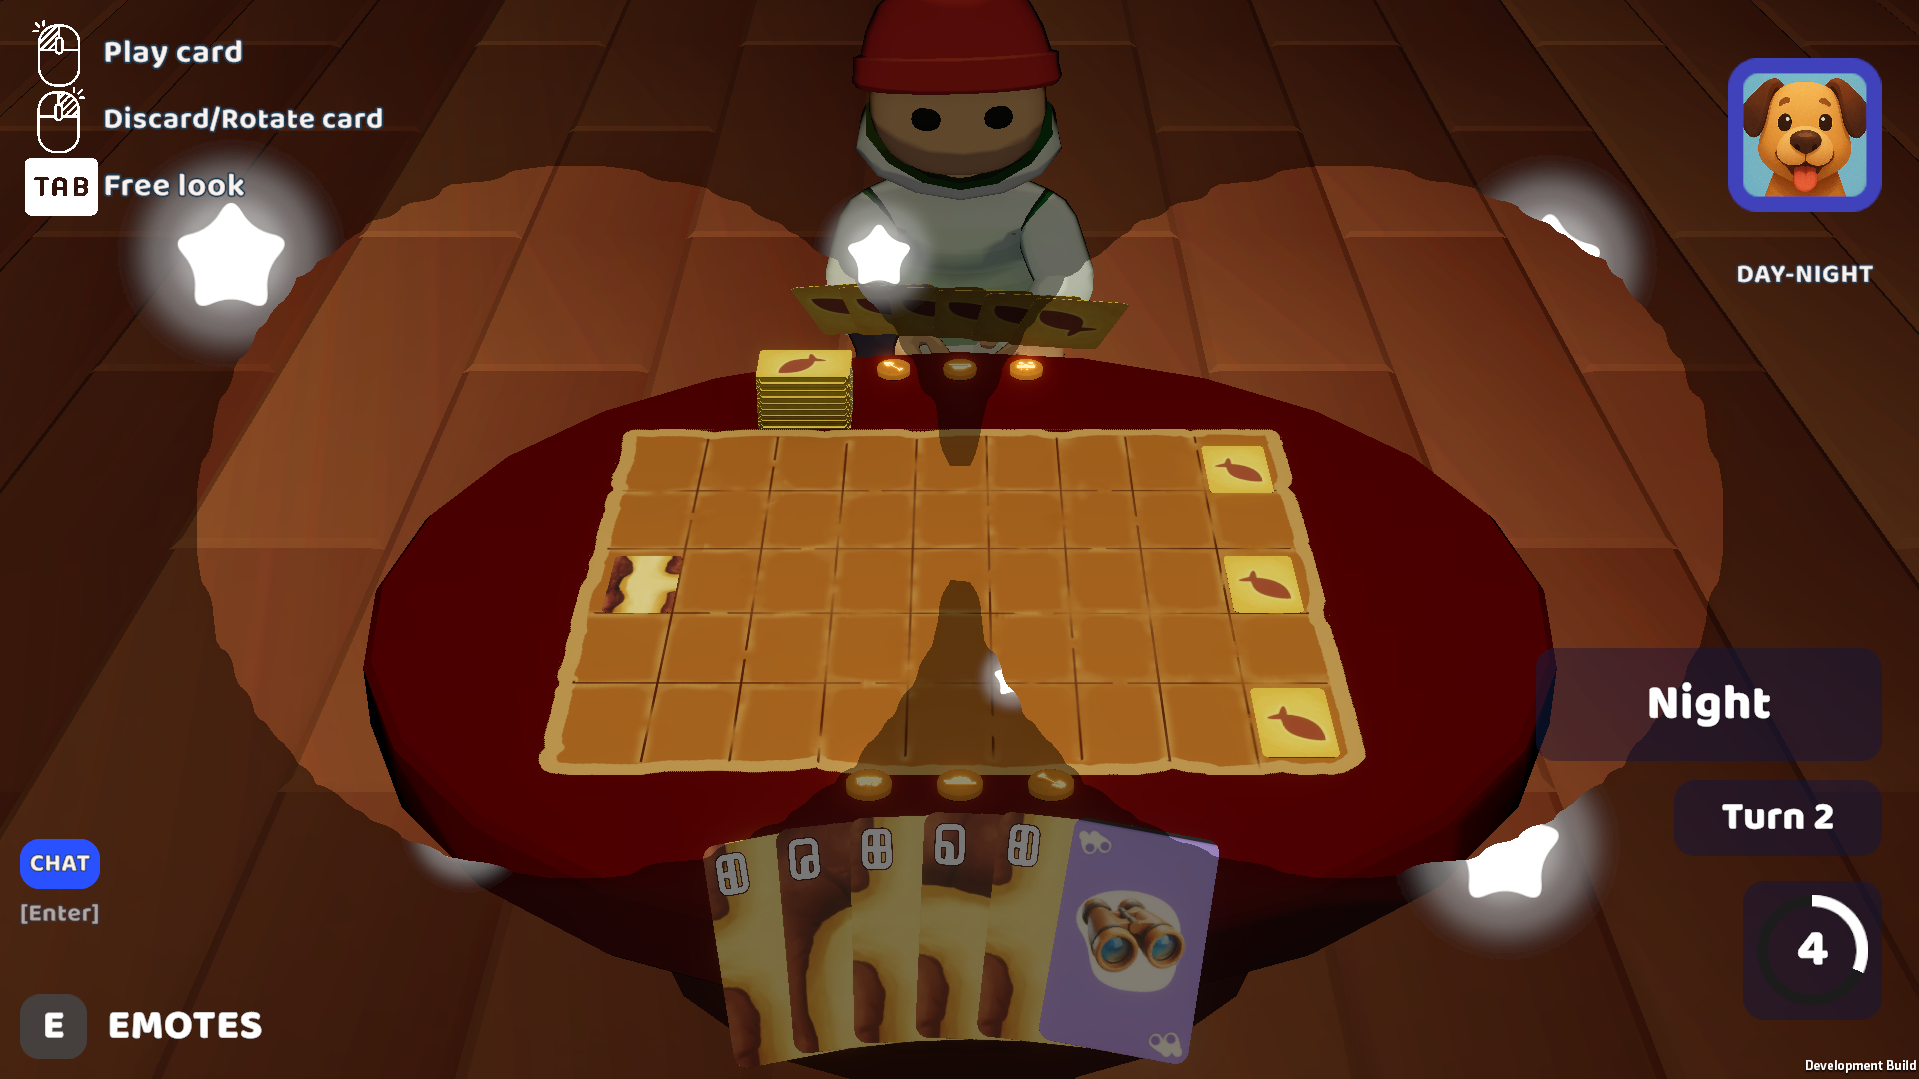
\includegraphics[width=0.5\linewidth]{10.Kết quả//images/Binocular.png}
    \caption{Screenshot sử dụng thẻ chức năng binoculars}
    \label{fig:placeholder}
\end{figure}

Sau khi đặt các thẻ đường sao cho có đường đến kho báu hoặc không còn thẻ bài nào trong tay bất kỳ người chơi nào thì sẽ kết thúc game đấu.
\begin{figure}[H]
    \centering
    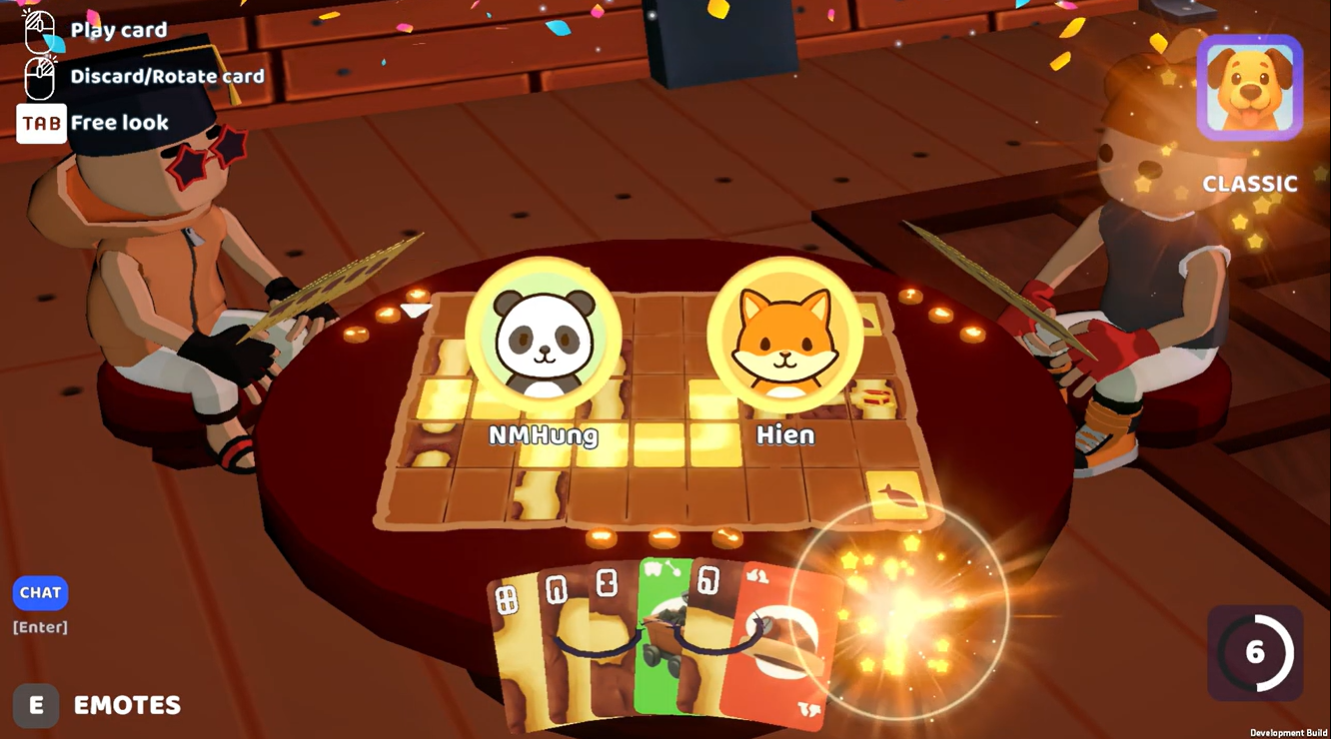
\includegraphics[width=0.5\linewidth]{10.Kết quả//images/victory.png}
    \caption{Screenshot màn hình \textbf{Chiến thắng}}
    \label{fig:placeholder}
\end{figure}